%- Hva karakterieserer plast utifra hva vi vet
%- ulike sensorer for deteksjon og kartlegging (vise sammenhengen til dette og en bredere oversikt - dette blir isåfall bare her, men tas ikke med videre - i metode kan vi heller si at vi avgrenser mot cam)
%- aktuelle sensorer 
%- sensorbærende plattform
%- PCA og singular value Decomp

%(alt dette kan evt komme kort i motivasjon) 


\section{Light}
%Color Registration of Underwater Images for Underwater Sensing with Consideration of Light Attenuation
%https://ieeexplore.ieee.org/stamp/stamp.jsp?tp=&arnumber=4209801
Light is electromagnetic radiation. The human eye can detect electromagnetic radiation within wavelengths of 400 and 750 nm, approximately. This electromagnetic spectrum is called visible light. Radiation with shorter wavelength than 400 nm is called ultraviolet, whereas infrared radiation has longer wavelength than visible light.

When light from a light source hits an object surface, the light is reflected before eventually reaching the eye. In this task, the endpoint will not only be the human eye, but other viewpoints, for instance a camera lens. The observation of the reflected colors in the viewpoint, is affected by properties of object surfaces, the light intensity of light source and traveling distance of the light.

Light in air behaves differently than in water. In air, the light will not be attenuated, which means that the reflection can be expressed by the light intensity, $I_ {\lambda}$ (eq \ref{eq:int}), describing the colors observed on the object.

\begin{equation} \label{eq:int}
    I_ {\lambda} (L, z) = \frac{S \cdot \kappa_{\lambda}\cdot cos^{3}\cdot (\alpha)}{z^2}
\end{equation}


In equation \ref{eq:int}, $I_{\lambda}$ represents the light intensity at a given wavelength, lambda, while S is the light source. L is the distance between the object and the viewpoint, while z describes the distance from the object to the light source. Furthermore, $\kappa_{\lambda}$ describes the reflectance ratio of the object's surface at a given wavelength, $\lambda$. $\alpha$ is the angle between the ray vector from the light source and the normal vector of the object surface.


\begin{figure}[H]
\centering
  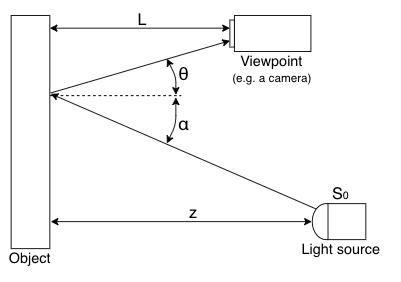
\includegraphics[width=12cm]{Images/theory/reflectance.png}
  \caption{Light refraction in liquid}
  \label{fig:reflectance}
\end{figure}



However, it is different if we do the same underwater. In water, light attenuation will be present and affect how the light is reflected.

\section{The Behavior of Light in Water}

%The light intensity decreases with the distance from objects in water by light attenuation depending on the wavelength of light. Red light decreases easier than blue light in water [E. O. Hulburt: “Optics of Distilled and Natural Water,” Journal of the Optical Society of America, Vol.35, pp.689–705, 1945].

The reason why the color of objects is different under water and in air, is that the light intensity, in water, decreases with the distance (r) to the object. This is, as mentioned, due to light attenuation, which again depends on the wavelength of the light. %([E. O. Hulburt: “Optics of Distilled and Natural Water,” Journal of the Optical Society of America, Vol.35, pp.689–705, 1945].) 
\\\\
From figure \ref{fig:lightinwater}, it can be observed that the intensity of the different colors decreases differently, even at the same distance, r. If the light source is 2 m away, red light will shine at half intensity, while blue light remains close to unchanged. At a distance of 20 meters, blue light will brighten at half-intensity. In this case, red and orange color will disappear.
%Color Registration of Underwater Images for Underwater Sensing with Consideration of Light Attenuation
%https://ieeexplore.ieee.org/stamp/stamp.jsp?tp=&arnumber=4209801

\begin{figure}[H]
\centering
  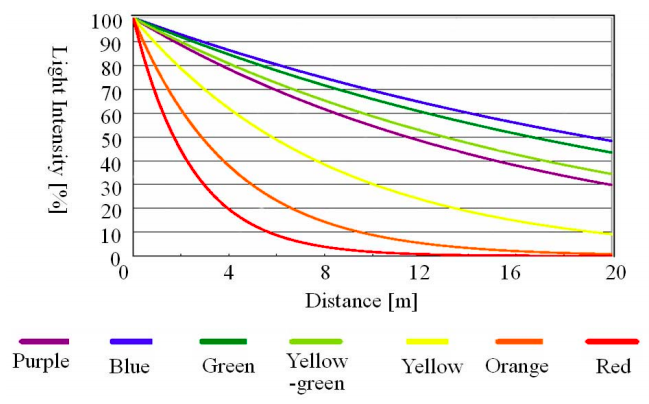
\includegraphics[width=12cm]{Images/theory/intensity.png}
  \caption{Light intensity in water.}
  \label{fig:lightinwater}
\end{figure}

As shown in the figure \ref{fig:lightinwater}, the light intensity decreases exponentially. The figure, is based on the following equation for the light source, S. 

\begin{equation} \label{eq:source}
S_{\lambda} (z) = S_0 \cdot exp (-c_{\lambda} \cdot r)
\end{equation}

In eq \ref{eq:source}, $S_{\lambda}$ describes the light intensity at wavelength $\lambda$, while $S_0$ is the intensity at the light source. Furthermore, r describes the distance between the light source and the viewpoint, while $c_{\lambda}$ is the attenuation coefficient of the wavelength $\lambda$, illustrated by figure \ref{fig:attcoeff}.
\\\\
By taking the attenuation coefficient, $c_{\lambda}$, into consideration, the light intensity in water can be expressed by the following similarity. 

\begin{equation} \label{eq:intw}
    I_ {\lambda} (L, z) = \frac{S \cdot \kappa_{\lambda}\cdot cos^{3}\cdot (\alpha)}{z^2} \cdot exp \left(-c_{\lambda}\left(\frac{z}{cos(\alpha)}\frac{L}{cos(\theta)}\right)\right)
\end{equation}

When interpreting eq \ref{eq:intw}, one can see that the intensity of light decreases when $c_{\lambda}$ increases. If $c_{\lambda} = 0$, meaning the light attenuation not being present, the resulting intensity becomes the same as the light intensity in air, eq \ref{eq:int}. 

\begin{figure}[H]
\centering
  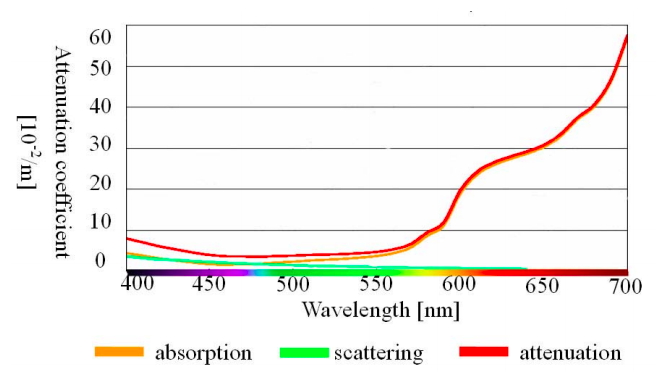
\includegraphics[width=12cm]{Images/theory/attcoeff.png}
  \caption{Attenuation coefficient}
  \label{fig:attcoeff}
\end{figure}


%Attenuation coefficient consists of absorption coefficient and scattering coefficient, because light attenuation consists of light absorption and light scattering. Attenuation coefficient of water changes very much with the wavelength of light. Consequently, observed colors changes in underwater environments.


%Stereo Measurement of Objects in Liquid and Estimation of Refractive Index of Liquid by Using Images of Water Surface
%http://www.robot.t.u-tokyo.ac.jp/~yamashita/paper/B/B047Final.pdf
Note: If cameras and objects are in the different condition where the refraction index differs from each other, several problems occur and a precise measurement cannot be achieved.

\section{Optical Fingerprints and Reflectance - IOP}
\todo[inline]{gå gjennom denne seksjonen + optical properties: Absorption and Scattering fra Silja}
%Underwater hyperspectral imaging: a new tool for marine archaeology 2018, ØYVIND ØDEGÅRD,1,2,* AKSEL ALSTAD MOGSTAD,3 GEIR JOHNSEN,3 ASGEIR J. SØRENSEN, AND MARTIN LUDVIGSEN1
Raw data consists of more than upwelling radiance reflected from the object. Reflections from the water column, ambient light and noise sensors are all parts of the data collected. However, the spectral reflectance reference is independent of the illumination and the water column properties. 

%Underwater hyperspectral imagery to create biogeochemical maps of seafloor properties 2013, G. JOHNSEN, NTNU
The spectral reflectance or ‘optical fingerprint’ can be described as a percentage of how much light at each wavelength is reflected off an object. Different objects absorb and reflect different wavelengths. In plants, red and blue wavelengths are highly absorbed, leaving the reflected color to be more or less green. Mathematically speaking, the spectral reflectance, $R(\lambda)$ is upwelling irradiance coming off the object, $Lu(\lambda)$, divided by the spectral downwelling irradiance towards the object, $Ed(\lambda)$.

%The use of underwater hyperspectral imaging deployed on remotely operated vehicles – methods and applications - geir og asgeir
\begin{equation} \label{eq:specref}
    R(\lambda) = \frac{Lu(\lambda)}{Ed(\lambda)}
\end{equation}

Where Lu(λ) denotes the raw data of the object, including signature from light source, while Ed(λ) is the spectral radiance from measurements of spectrally neutral reflectance standard.

Note: For eq \ref{eq:specref} to hold true, all surfaces are assumed to behave like Lambertian reflectors. 
%The use of underwater hyperspectral imaging deployed on remotely operated vehicles – methods and applications - geir og asgeir

\subsection{IOP}


\section{The Digital Image}
%evt Fysikken bak bildet 
%Info hentet fra bok: techniques and applications of hyperspectral image analysis

From the mid-20th century, images have been stored in digital format (Geladi and Grahn, 2000). A digital image is an array of rows (i) and columns (j) consistent of i x j gray-values. A gray-value, better known as an intensity or a pixel, is simply one of many small squares in an image. If the image is to consist of colors however, a third dimension is needed. This dimension is shown as the depth in FIGURE.. The depth is three intensities/layers deep, consisting of red, green and blue. What was previously a gray pixel is now a voxel, a triplet of red, green and blue.
\\\\
One can say that a color image has three layers, red, green and blue, each of which contains different information. However, if the interval separating the layers is chosen to be a shorter wavelength, the number of layers will increase. The resulting image is then called a multivariate image. If k denote the depth dimension and thus determine the number of wavelengths which in turn will constitute the number of layers, the resulting array will be of the size i x j x k. FIGURE!
\\\\
For a human eye to be able to perceive a color image, only three wavelengths / layers are needed, namely red, green and blue. It therefore rarely makes sense to create multiple layers unless the goal is to capture information the eye cannot see. This is where hyperspectral imaging enters the playing field, which by definition has more than 100 layers and can express each pixel as a spectrum.

\begin{figure}[H]
  \newcommand*\FigVSkip{0.5em}
  \newcommand*\FigHSkip{0.1em}
  \newsavebox\FigBox
  \centering
  % Top image is centered, so no need to get width
 \sbox{\FigBox}{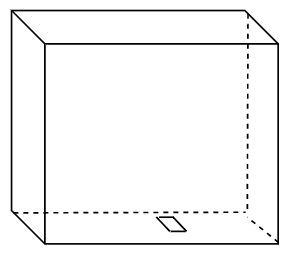
\includegraphics[scale=0.5]{Images/theory/pixel.png}}
  \begin{minipage}{\wd\FigBox}
    \centering\usebox{\FigBox}
    \subcaption{a) Pixel}
  \end{minipage}
  % Save first image in a box to get the width
  \sbox{\FigBox}{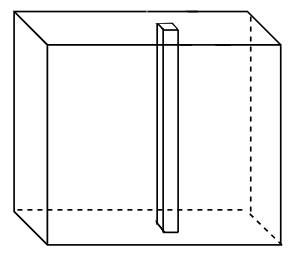
\includegraphics[scale=0.5]{Images/theory/voxel.png}}
  \begin{minipage}{\wd\FigBox}
    \centering\usebox{\FigBox}
    \subcaption{b) Voxel}
  \end{minipage}\hspace*{\FigHSkip}
  % Save second image 
  \label{head}
\end{figure}

\section{Imaging Process}
%Denne skal jeg få tilsendt av Asgeir

\section{Hyperspectral Imaging}
%Use of Underwater Hyperspectral Imager (UHI) in Marine Archaeology 2014, Øyvind Ødegård1,3, Geir Johnsen2 and Asgeir J. Sørensen1

Hyperspectral imagery is defined as images that contain a spectrum of reflected light with a spectral resolution of 1-5 nm per image pixel (4). Materials or compositions of materials (object of interest, OOI) will absorb, scatter and reflect light of different portions of the visible spectrum, giving them their own optical fingerprints that are unique, and can be used for classification with high degree of confidence (4). 

%Info hentet fra yt
In order to study the reflecting light from the target, one need a spectrometer. A spectrometer is an instrument that splits the incoming light into a spectrum. Measuring this reflectance spectra is the most common way to use hyperspectral imaging.
\\\\
Hyperspectral imaging uses an imaging spectrometer (also called a hyperspectral camera) to collect spectral information. As mentioned, the difference between a hyperspectral image and a regular photo, is that the hyperspectral camera measures hundreds of thousands of spectra instead of single spectrum, creating a multispectral image. But in contrast to multispectral imagers, which are sensitive in only a few selected wavebands, hyperspectral imagers (HI) measure the spectral upwelling radiance Lu(λ) or reflectance R (λ) per image pixel of bio-geo-chemical object of interest (Klonowski et al. 2007; Volent et al. 2007; Johnsen et al. 2009, 2013b). %(Development of hyperspectral imaging as a bio-optical taxonomic tool for pigmented marine organisms - geir)

This way, the resulting image of the target includes a complete spectrum for each pixel in the image. By doing this, it is possible to determine what the image is actually showing. 

\\\\
%The spectral information in every pixel creates a third dimension, providing a collection of data called a data cube. Now, how does this data differ from the data and images from other types of cameras? Digital camera, shoots the target in red, green and blue, in order to match the human vision. These camera leaves a combination of the three colors, which is what we can see with our eyes. This means that the information constituting the third dimension consists of nothing more than three colors, while the hyperspectral camera records hundreds of wavelengths. This way, the hyperspectral camera can collect more detailed information about the target, not only in visible light, but also in infrared and ultra violet. By combining different wavelengths, pixel by pixel, one can extract useful information about the properties of the target. 




%Hyperspectral imaging and data analysis for detecting and determining plastic contamination in seawater filtrates, 2016,  Bert van Bavela
%http://journals.sagepub.com/doi/pdf/10.1255/jnirs.1212
Concerning plastics, this translates to receiving information on both spatial location of plastic material, and the plastic materials composition. 
%Volent, Z., Johnsen, G., & Sigernes, F. (2007). Kelp forest mapping by use of airborne hyperspectral imager. Journal of Applied Remote Sensing, 1, 011503–011521.
%Volent, Z., Johnsen, G., & Sigernes, F. (2009). Microscopic hyperspectral imaging used as a bio-optical taxonomic tool for micro- and macroalgae. Applied Optics, 48, 4170–4176.

%(Development of hyperspectral imaging as a bio-optical taxonomic tool for pigmented marine organisms - geir)
HI and UHI can be used as a taxonomical identification tool to make optical fingerprints of marine organisms only if the pigment composition and corresponding absorption signature of the organism is known and can be used to verify the reflectance signature

When the hyperspectral camera is taken underwater, the lighting is limited. The UHI is therefore using its own light sources, in contrast to passive passive techniques using ambient light (Johnsen et al. 2013b).
%(Development of hyperspectral imaging as a bio-optical taxonomic tool for pigmented marine organisms - geir) %The use of underwater hyperspectral imaging deployed on remotely operated vehicles – methods and applications - geir og asgeir


%Info hentet fra bok: techniques and applications of hyperspectral image analysis
 %oppsettene inkluderer lyskilde, et filtersystem som disperse the light into bands of wavelenghts, en sample. Hvis kilden inneholder et bredt lysspekter, kan man velge ut bølgelengder ved å bruke bandpass-filters etter ønske.
\\\\In this task, there are two methods for camera configurations, point scanning image and line scanning image.
\subsection{Point Scanning Image}
Point scanning image can be used to measure a complete spectrum in one spot/pixel. In every spot, all layers are measured vertically from this spot. To make the whole picture, the camera must scan across the entire surface, spot by spot.
\\\\
figuren er hentet fra boken, techniques and applications of hyperspectral image analysis, side 6

% \begin{figure}[H]
%   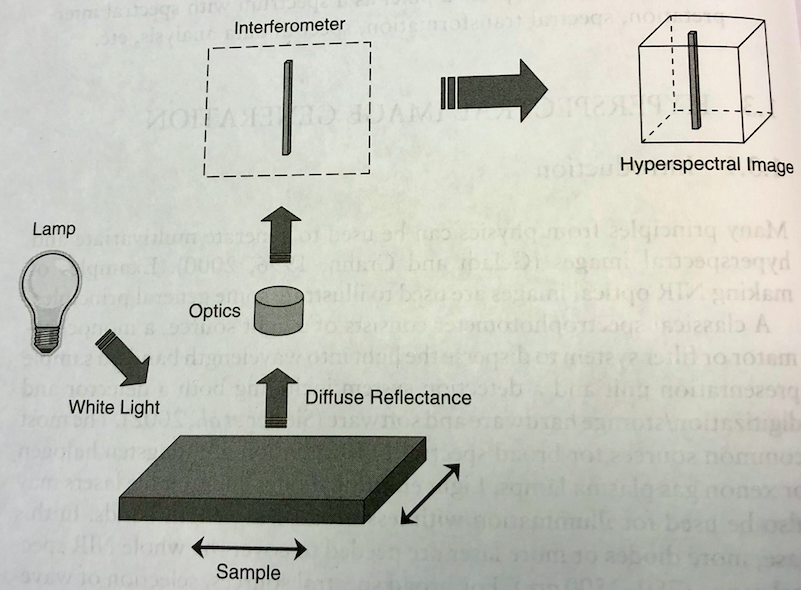
\includegraphics[height=12cm]{Images/theory/pointscan.png}
%   \caption{Set-up, Point Scanning Image}
%   \label{fig:pointscan}
% \end{figure}


\begin{figure}[H]
\centering
  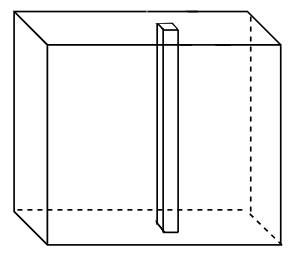
\includegraphics[height=6cm]{Images/theory/voxel.png}
  \caption{Resulting scan}
  \label{fig:voxel2}
\end{figure}


\subsection{Line Scanning Image}
The line scanning image technique uses a two-dimensional detector, perpendicular/orthogonal to the surface of the measured target. This detector collects the spectrum of a whole line in the image, in one single scan. By moving the scan line with a push broom technique, one can map the entire image by combining all sets of spectra.
\\\\
figuren er hentet fra boken, techniques and applications of hyperspectral image analysis, side 7

% \begin{figure}[H]
% \centering
%   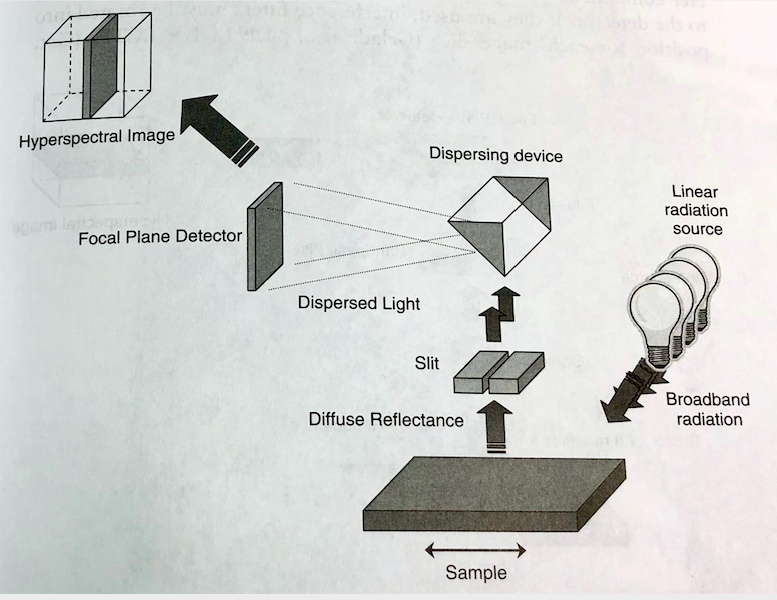
\includegraphics[height=12cm]{Images/theory/linescan.png}
%   \caption{Set-up, Line Scanning Image}
%   \label{fig:linescan}
% \end{figure}

\begin{figure}[H]
\centering
  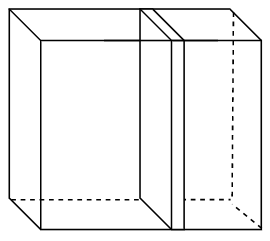
\includegraphics[height=6cm]{Images/theory/pushbroom.png}
  \caption{Resulting scan}
  \label{fig:pushbroom}
\end{figure}

\section{Geo Reference}


\section{Silhouette Camera}
https://github.com/emlynjdavies/PySilCam/wiki 



\section{Microplastic}
%ha med hva def av mikroplast og de ulike plasttypene
Kjemi

As mentioned, plastics have permeated almost every aspect of modern day life with its large applicability. We find plastics in the microchips in our computers, as well as in the bags we carry our groceries in. It seems that plastic covers a wide spectrum of applications.  One reason to this, is the many different types of plastic, covering different areas of need. Polyethylene (PE), polypropylene (PP), polyethylene terephthalate (PET), polyvinyl chloride (PVC) and polystyrene (PS), are the five most common types of plastic, covering a large \todo{hvor mye? kan summere opp alle prosentene fra wiki: 34 + } percent of the global plastic production. Besides containing Carbon-Hydrogen bindings, these are all structurally different and they are classified according to their chemical structure. 

%Plastic polymers commonly found in the environment are polypropylene (PP), polyethylene (PE), polyethylene terephthalate (PET), polystyrene (PS) and polyvinylchloride (PVC).8 Together these comprise 72.9 percent of the plastic produced globally.9

\subsection{Polyethylene}
The molecules in polyethylene (PE) has the chemical formula C2H4 \todo{figur av struktur}. Polyethylene is the most common type of plastic, with 34\% of all plastic produced being PE. The reason to its commonness is the broad application of it in consumer products. Plastic bags, bottles and food wrapping are good examples of polyethylene. However, these three products seem to have a significantly different material. For instance are plastic bags rarely as rigid and as bottles. This variation in polyethylene creates two sub-types defined by the degree of density – HDPE and LDPE, high-density polyethylene and low-density polyethylene respectively. 

The LPDE-molecules are more branched, meaning that a chain is replacing for instance a hydrogen atom. As a result of this, the molecules are less tightly packed, leading to a lower density.  As LDPE has more branching than HDPE, its intermolecular forces are weaker. \todo{FIGUR av branch-forskjellene!}


\subsection{Polypropylene}
Polypropylene (PP) is the second most common plastic consistent of propylene with the chemical formula C3H6. PP has properties similar to polyethylene, but it is slightly harder and more resistant to fatigue. The plastic type is found in a variety of products like food packaging, labeling and clothing. 

\subsection{Polyvinyl Chloride}
%http://www.plasticmoulding.ca/polymers/pvc.htm
Polyvinyl chloride (PVC) with a number of vinyl chloride molecules formulated by C2H3Cl, is in third place of the most produced types of plastic. PVC can be both rigid and flexible. The rigid form is used in constructional application in piping and electrical wire insulation, while the softer and more flexible form is used in many applications replacing rubber. 

\subsection{Polyethylene terephthalate (PET)}
Polyethylene terephthalate (PET): Commonly known as polyester. One of the most widely used type of plastic. It is used in a wide range of articles, from plastic bags to clothing and beverage containers.

\subsection{Polystyrene (PS)}
Polystyrene (PS): An inexpensive type of polastic and is therefore often used in disposable plastic objects, such as cutlery, containers and other types of packaging



\section{Principal Component Analysis}

The purpose of conducting a principal component analysis is to extract the information from the data, while disregarding the noise, reducing the dimension of the dataset. The analysis converts a set of observations of possibly correlated variables into a set of values of linearly uncorrelated variables called principal components. These principal components will describe the overall variation of the dataset and thereby serve as a latent variable. 
\\\\
Now, how are these principal components found? Figure a) below describes the entire dataset with the dots describing single data observations. The analysis starts by finding the projection of each observation onto a line. The line is drawn with the purpose of explaining as many observations as possible with a minimal residual error, b). The distance from the origin to this projected point along the line is the score associated with the related observation. The direction of the line is now characterized with giving the largest variance of the scores, and is described by direction vectors called loadings. 
\\\\
%Simply put, the original data is estimated by multiplying the scores with the associated loadings.
This first line created is called the first principal component. The second principal component, c), is perpendicular to the first component’s direction and is otherwise found the same way. This way, the first principal component has the largest possible variance. Each following component will, in turn, have the highest variance possible under the constraint that it is perpendicular to the previous components. 

%FIGURENE:
%https://learnche.org/pid/latent-variable-modelling/principal-component-analysis/geometric-explanation-of-pca
\begin{figure}[H]
  \newcommand*\FigVSkip{0.5em}
  \newcommand*\FigHSkip{0.1em}
  \newsavebox\FigBox
  \centering
  % Top image is centered, so no need to get width
\sbox{\FigBox}{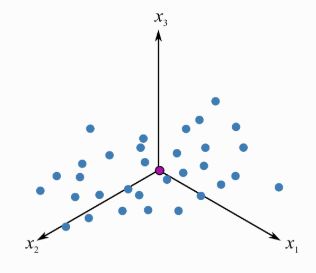
\includegraphics[scale=0.4]{Images/theory/koord.png}}
  \begin{minipage}{\wd\FigBox}
    \centering\usebox{\FigBox}
    \subcaption{a) Scaled and centered data observations}
  \end{minipage}
 \sbox{\FigBox}{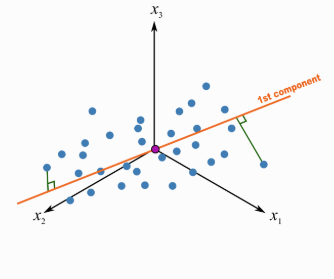
\includegraphics[scale=0.4]{Images/theory/1pc.png}}
  \begin{minipage}{\wd\FigBox}
    \centering\usebox{\FigBox}
    \subcaption{\newline b) Including first principal component}
  \end{minipage}
  % Save first image in a box to get the width
  \sbox{\FigBox}{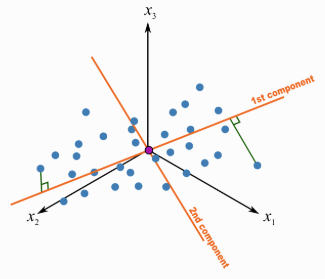
\includegraphics[scale=0.4]{Images/theory/2pc.png}}
  \begin{minipage}{\wd\FigBox}
    \centering\usebox{\FigBox}
    \subcaption{c) Including second principal component}
  \end{minipage}\hspace*{\FigHSkip}
  % Save second image 
  \label{head}
\end{figure}



\todo[inline]{Skrive om den under til både forsøksrelevant og ny}
%Underwater hyperspectral imaging: a new tool for marine archaeology 2018, ØYVIND ØDEGÅRD,1,2,* AKSEL ALSTAD MOGSTAD,3 GEIR JOHNSEN,3 ASGEIR J. SØRENSEN, AND MARTIN LUDVIGSEN1
To assess the spectral relationship between different objects and materials, principal component analyses were performed on the laboratory-acquired reflectance data. The principal components can be seen as the axes in an ellipsoid with n dimensions that describes the data. The longest axis accounts for the largest variance in the data, and corresponds to principal component 1 (PC1). The second-longest axis corresponds to PC2, and so on.

\subsection{Scores, Loadings, F-residuals, Hotellings T^2 }
https://learnche.org/pid/latent-variable-modelling/principal-component-analysis/interpreting-the-residuals

\section{Sensor Carrying Platform}
%ulike sensorer for deteksjon og kartlegging (vise sammenhengen til dette og en bredere oversikt - dette blir isåfall bare her, men tas ikke med videre - i metode kan vi heller si at vi avgrenser mot cam. + aktuelle sensorer







%\subsection{General behavior changes in water}
%\subsection{Lysets oppførsel i vann}